\section{Estruturas de RNA}
RNA podem apresentar vários tipos de estrutura, dado sua capacidade de ligar neurônios artificiais. Como estruturas de sistemas nervosos biológicos, cada estrutura distinta de RNA pode ser especializada em problemas específicos. Nesse sentido vale-se a discussão que não necessariamente uma rede com uma quantidade grande de neurônios e ligações será melhor que uma rede com poucas ligações e menor números de neurônios dado alguma aplicação especifica.

Um neurônio artificial é modelado tendo terminais de entradas\textit{x} e um terminal de saída.O comportamento das sinapses é simulado através dos pesos aplicados nas entradas do neurônio, a saída do neurônio é dada por : 
\begin{equation}
Sj = \theta *\sum_{i=0}^{m} (wij*xi+bj)
\end{equation}

Onde $\theta$ representa a função de ativação, \textit{bj} corresponde ao \textit{bias}, \textit{pij} são os pesos sinápticos[5].
\begin{figure}[H]

\centering % para centralizarmos a figura
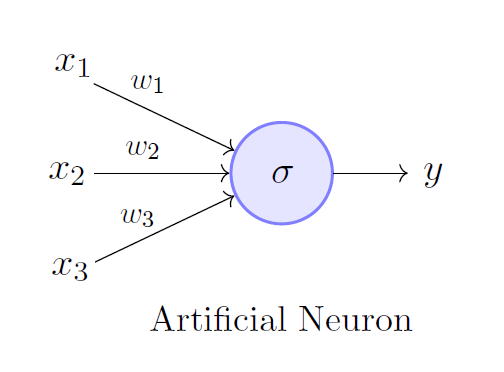
\includegraphics[width=\columnwidth]{04-Figuras/fig}
\caption{Estrutura de um neurônio artificial}

\label{figura:arquitetura}

\end{figure}
De forma geral uma rede neural é constituída de unidades simples de processamento denominadas de neurônios e ligações massivas entre essas unidades.[5]
Mais a frente nessa seção será detalhado a constituição de Redes MLP e anociassociativos competitivas


\subsection{Perceptrom de Multiplas Camadas}
A rede perceptron de múltiplas camadas como o próprio nome indica apresenta várias camadas em sua estrutura,tendo como composição mínima uma camada de entrada, uma camada de saída e uma camada intermediária. Segundo o modelo descrito por [5], essas camadas são ligadas por sinapses com pesos(\textit{pij}) intrínsecos, assim compondo uma rede vasta de interconexões regidas por pesos e funções de ativação.
\begin{figure}[H]

\centering % para centralizarmos a figura
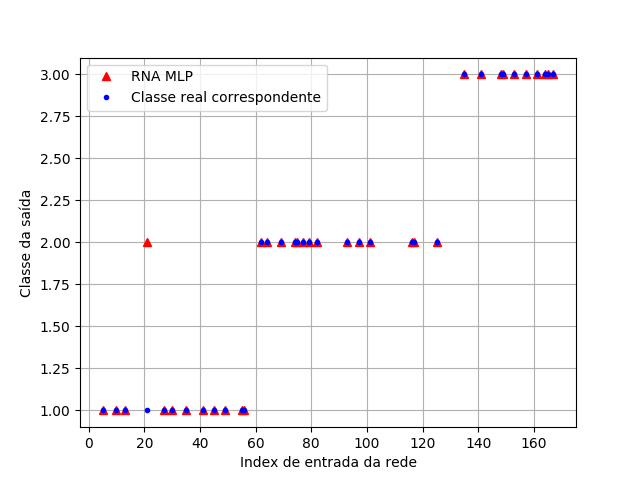
\includegraphics[width=\columnwidth]{04-Figuras/MLP}
\caption{Estrutura de um neurônio artificial}

\label{figura:Arquitetura de uma rede MLP}

\end{figure}

O aprendizado da MLP consiste em 2 passos, o passo direto e o passo inverso. O passo direto ou \textit{forward pass} consiste em passar as entradas pela rede, assim aplicando os pesos associados as sinapses, e obtendo assim a saída. O segundo passo consiste na retropropagação do erro, é calculado o gradiente da função de perda na camada de saída, posteriormente esse gradiente é utilizado para aplicar recursivamente a regra da cadeia para atualizar os pesos de toda a rede.
Esse algorítimo é chamado de \textit{backpropagation}[1].

\subsection{Redes Autoassociativas competitivas}
Redes neurais do tipo autoassociativas ou \textit{autoencoders} baseiam-se em MPL que apresentam o mesmo número de neurônios na camada de entrada e na camada de saída, a camada intermediária apresenta um número inferior de neuronios em relação as outras duas camadas. 

A estrutura da camada de entrada juntamente com a camada intermediária funcionam como um encoder, também chamada de gargalo, comprime a informação inserida na entrada. 

A estrutura de saída juntamente com a camada intermediária funciona como um decoder, descomprimindo a informação obtida da camada intermediária.Dessa maneira, a rede  tenta recriar os dados que foram inseridos na entrada[6].
\begin{figure}[H]

\centering % para centralizarmos a figura
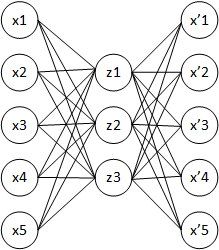
\includegraphics{04-Figuras/autoencoder}
\caption{Estrutura de rede autoencoder}

\label{figura:arquitetura}

\end{figure}

A estrutura competitiva baseia-se em criar e treinar um numero de redes autoencoders igual ao número de classes do problema de classificação, de forma a criar redes especializadas em recriar os dados de entrada de inseridos para cada classe. Dessa forma, as redes treinadas para uma dada classe irão apresentar um erro médio quadrático menor ao serem inseridos dados da classe a qual foram treinadas.

Após o treinamento essas redes são colocadas lado a lado, recebendo as mesmas entradas e tentando recria-las.Posteriormente, mede-se o erro quadrático médio de cada rede para cada índice de entrada, os valores de erro são avaliados e infere-se a classe de saída correspondente a rede que apresentou o menor erro na recriação dos dados de entrada[6].Dessa maneira as redes competem entre si para assim gerar um valor de classe na saída.


%=================================================================================================
\section{Banco de Dados}
A base de banco de dados de vinho selecionada para a produção desse artigo foram resultados de uma análise química de vinhos cultivados na mesma região da Itália,mas derivados de três diferentes cultivares[2].

Os atributos de entrada da rede são Álcool, Acido málico, Cinzas,Alcalinidade das cinzas , Magnésio,Fenóis totais,Flavonoides,Fenóis não flavonoides,Proantocianidinas,Intensidade da cor, tonalidade,OD280 / OD315 de vinhos diluídos e Prolina.

A base de dados foi organizada de forma que cada grupo de 13 variável tem um índex associado e uma classe correspondente.

\begin{table}[H]
\centering
\caption{Distribuição da base de dados}
\begin{tabular}{ccccc}
\hline

\multicolumn{1}{l}{Faixa de Index} & \multicolumn{1}{l}{Classe correspondente} \\ \hline
\textit{0-58}                      & 1                                         \\
58-129                             & 2                                         \\
131-77                             & 3                                         \\ \hline
\end{tabular}%

\label{tabela:baseDados}

\end{table}


 A divisão da base de dados em dados de treino, validação e teste foi realizada com a biblioteca Scikit[7], a qual randomiza a seleção de índex para a divisão do banco de dados em dada proporção previamente programada. A proporção utilizada para a divisão consta na Tabela 2.

\begin{table}[H]
\centering
\caption{Divisão da base de dados}
\resizebox{\columnwidth}{!}{%
\begin{tabular}{cccccccc}
\hline
Distribuição dos dados & \multicolumn{2}{c}{\begin{tabular}[c]{@{}c@{}}Classe 1\\ n        \%\end{tabular}} & \multicolumn{2}{c}{\begin{tabular}[c]{@{}c@{}}Classe 2\\ n        \%\end{tabular}} & \multicolumn{2}{c}{\begin{tabular}[c]{@{}c@{}}Classe 3\\ n        \%\end{tabular}} & Total de Dados \\ \hline
Treino & 35 & 60\% & 44 & 60\% & 27 & 60\% & 106 \\
Validação & 12 & 20\% & 14 & 20\% & 10 & 20\% & 36 \\
Teste & 12 & 20\% & 14 & 20\% & 10 & 20\% & 36 \\ \hline
\end{tabular}
}
\end{table}

 
%=================================================================================================
\section{Desenvolvimento da Rede MLP}
A rede MLP foi desenvolvida em Python[3] com o auxilio da bibliotecas Keras[4].A divisão de dados em treino validação e teste foi seguido como está proposto na Tabela 2, e apesar de que a escolha dos índex de conjunto de entradas é feito de forma randômica, foi fixado duma \textit{seed} na biblioteca Scikit[7], de forma a sempre ser executada a mesma divisão de dados.

A estrutura da rede apresenta 3 camadas, na camada de entrada exite 13 neurônios para receber os dados, a camada de saída dispõe de apenas 1 neurônio. Para definir o numero óptimo de neurônios na camada intermediária foi realizado um levantamento da acurácia com relação a esse numero.

\begin{figure}[H]
\centering % para centralizarmos a figura
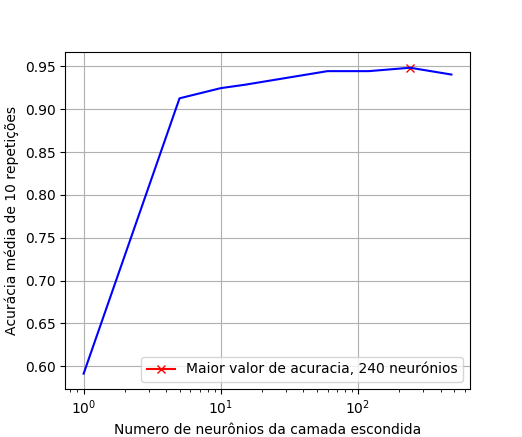
\includegraphics[width=\columnwidth]{04-Figuras/acuracia}
\caption{Acurácia vs Nº de neurônios na camada escondida}
\label{figura:acuracia}
\end{figure}

Depois de definido o número de neurônios da camada escondida, os dados utilizados no treino validação e  teste foram normalizados, de forma que cada coluna dos 13 atributos foi dividida pelo maior número da coluna.

A função de ativação da camada escondida escolhida foi \textit{sigmoid},a função de ativação da camada de saída foi linear, a escolha das funções foi feita depois de vários testes de desempenho relacionando o erro com a função de ativação escolhida.

A saída da rede foi arredondada para o inteiro mais próximo, por conta que o este tratava-se de um número fracionário.Dessa forma, após realizar a aproximação, o valor de saída enquadra-se em alguma das 3 classes presentes no banco de dados.

\section{Desenvolvimento da Rede Autoencoder competitiva}
Assim como a Rede MLP, a  rede autoencoder competitiva foi desenvolvida utilizando os mesmo software e bibliotecas.A divisão dos dados de entrada em treino validação e teste ocorreu de forma idêntica a rede MLP construída anteriormente.

Feito a divisão de dados de treino de todas as 3 classes, essa foram criadas 3 MLP conectadas de forma competitiva[6]. Essas redes contavam com 13 neurônios na camada inicial e na camada de saída, na camada intermediária foi executado a análise do número de neurônios versus a acurácia total da rede competitiva para descobrir o valor ideal de neurônios na camada intermediária.

\begin{table}[H]
\centering
\caption{Distribuição da base de dados}
\begin{tabular}{cc}
\hline
\begin{tabular}[c]{@{}c@{}}Nº de neurónios na \\ \\ camada escondida\end{tabular} & \begin{tabular}[c]{@{}c@{}}Acurácia média \% \\ \\ de 10 repetições\end{tabular} \\ \hline
1 & 94.44444444 \\
4 & 100 \\
8 & 91.11111111 \\
12 & 69.16666667 \\ \hline
\end{tabular}

\label{tabela:baseDados}

\end{table}


A função de ativação escolhida visando a maior acurácia da rede foi linear tanto na camada escondida quanto na camada de saída.